\documentclass[a4paper,12pt,draft]{scrreport}

\usepackage[lang=de,lib=false]{../general/preamble}

\begin{document}

\begin{titlepage}
    \begin{center}
        \vspace*{1cm}
 
        \Large{\textbf{Der Morse-Komplex und die Morse-Homologie}}
 
        \vspace{0.5cm}
        Eine Bachelorarbeit \\ 
        Betreuerin Prof. Ursula Ludwig
             
        \vspace{1.5cm}
 
        \textbf{Jakob Dimigen}
             
    \end{center}
\end{titlepage}

\tableofcontents

\begin{abstract}
    In der Morse Theorie werden glatte Abbildungen $f \colon M \to \R$, deren kritische Punkte 
    alle nicht degeneriert sind untersucht. Anhand einer solcher Abbildungen lassen sich
    Rückschlüsse auf topologische Eigenschaften der Mannigfaltigkeit $M$ ziehen. In dieser Arbeit
    wird der \textit{Morse-Komplex} definiert, und gezeigt, dass dieser isomorph zu einem zellulären 
    Kettenkomplex ist. Dafür wird anfangs eine kurze Einführung in die Morse-Theorie gegeben und 
    grundlegende Begriffe definiert. Im zweiten Kapitel werden Morse Funktionen und Pseudo-Gradienten 
    untersucht. Im dritten Kapitel wird bewiesen, dass der Morse Komplex ein Kettenkomplex ist und 
    im letzten Kapitel wird anhand der erarbeiteten Theorie eine zelluläre Struktur auf kompakten 
    Mannigfaltigkeiten konstruiert, deren zellulärer Kettenkomplex isomorph zum Morse-Komplex ist.
    Zu guter letzt werden einige bekannte Eigenschaften der zellulären Homologie anhand der 
    Morse Homologie bewiesen. Something something
\end{abstract}

\label{somesection}

\include{ch1-einführung}

\chapter{Morse-Funktionen und Pseudo-Gradienten}

Das Ziel dieses Kapitels ist es, Morse-Funktionen und Pseudo-Gradienten zu
definieren und ihre \todo{allgegen- wertigkeit ist nicht so ein schönes Wort}
\textit{allgegenwertigkeit} zu zeigen. Ein weiteres wichtiges Ergebnis ist
das \textit{Morse-Lemma}.

\section{Morse-Funktionen}

In diesem Abschnitt untersuchen wir \textit{Morse-Funktionen}:

\begin{definition}[Morse-Funktion]
    \label{satz: morse-funktion}
    Eine \textit{Morse-Funktion} auf einer glatten Mannigfaltigkeit $M$ ist eine glatte Funktion
    $f \colon M \to \R$, deren kritische Punkte alle nicht degeneriert sind.
\end{definition}

Insbesondere zeigen wir, dass Morse Funktionen nichts besonderes sind. Dafür zeigen wir, dass für 
eine Untermannigfaltigkeit $M \subseteq \R^n$ und einen Punkt $p \in \R^n$ die Abbildung
$x \mapsto \| x - p \|^2$ nur für $p$, die so gennanten \textit{Brennpunkte}
sind, keine Morse Funktion ist.

\begin{definition}[Normalenbündel]
    \label{def: normalenbuendel}
    Es sei $M \subseteq \R^n$ eine Untermannigfaltigkeit von $\R^n$. Das Normalenbündel ist die 
    Menge
    \[ NM = \{ (x, v) \in M \times \R^n : v \perp T_xM \} . \]
    Wir betrachten hier $T_xM \subseteq T_x\R^n \isom \R^n$ via der Basis 
    $\left( \del / \del x_i \right)$, wobei $x_i$ die Achsen des $\R^n$ sind.
\end{definition}

\begin{prop}
    \label{prop: NM ist untermannigfaltigkeit}
    Das Normalenbündel $NM$ ist eine $n$-dimensionale Untermannigfaltigkeit von $M \times \R^n$.
\end{prop}

\begin{proof}
    Es sei $x \in M$. Dann existiert eine Umgebung $U \subseteq \R^n$ von $x$, eine Umgebung 
    $\Omega \subseteq \R^d$ von $0$ und eine Immersion 
    \begin{align*}
        h \colon \Omega \longto & \R^n \\
        (u_1, \dots, u_d) \; \longmapsto & \; x(u_1, \dots, u_d)
    \end{align*}
    die ein Diffeomorphismus $h \colon \Omega \to U \cap M$ ist. Das orthogonale Komplement 
    von $T_xM$ in $\R^n$ hat Dimension $n - d$. Es sei also 
    $(v_1(x), ..., v_{n-d}(x))$ eine Basis von $(T_xM)^{\perp}$. Dann ist 
    \[ (u_1, ..., u_d, t_1, ..., t_{n - d}) \longmapsto 
        \left(x(u_1, ..., u_n), \sum_{k = 1}^{n - d} t_k \cdot v_k(u_1, ..., u_d)\right) \]
    eine lokale Parametrisierung von $NM$ als Untermannigfaltigkeit von $M \times \R^n$.
\end{proof}

\begin{definition}[Brennpunkt]
    \label{def: brennpunkt}
    Es sei $M \subseteq \R^n$ eine Untermannigfaltigkeit von $\R^n$. Es sei $E \colon NM \to R^n$ 
    mit $E (x, v) = x + v$. Ein \textit{Brennpunkt} von $M$ ist ein kriticher Wert von $E$.
\end{definition}

\begin{remark}
    Aus dem Satz von Sard folgt, dass die Menge der Brennpunkte eine Nullmenge ist.
    Intuitiv sind die Brennpunkte einer Untermannigfaltigkeit die Punkte im $\R^n$, an denen sich
    die Normalen von nahe aneinanderliegenden Punkten schneiden.
\end{remark}

\begin{lemma}
    \label{lemma: char. von Brennpunkten}
    Es sei $M \subseteq \R^n$ eine Untermannigfaltigkeit von $\R^n$ $x \in M$ und $M$ in einer 
    Umgebung von $x$ und $NM$ parametriesiert wie im Beweis von 
    Proposition~\ref{prop: NM ist untermannigfaltigkeit}. Dann ist $p = x + v$ genau dann ein
    Brennpunkt von $M$, wenn die Matrix 
    \[
        \left( \left\langle \pderive[x]{u_j}, \pderive[x]{u_i} \right\rangle - 
        \left\langle v , \pdderive[x]{u_i}{u_j} \right\rangle \right)_{ij}
    \]
    nicht invertierbar ist.
\end{lemma}

\begin{proof}
    Wir haben partielle Ableitungen
    \[ \pderive[e]{u_i} = \pderive[x]{u_i} + \sum_{k = 1}^{n - d} t_k \pderive[v_k]{u_i} \]
    und 
    \[ \pderive[E]{t_j} = v_j \]
    Nun ein kleines Ergebnis aus der Linearen Algebra:

    sind $v_1, ..., v_n, u_1, ..., u_n \in \R^n$ und $u_1, ..., u_n$ linear unabhängig, 
    dann ist
    \[ (v_1 \; ... \; v_n)^T \cdot (u_1 \; ... \; u_n) = (\langle v_i, u_j \rangle)_{ij} , \]
    Also 
    \[ \rank (v_1 ... v_n) = \rank (\langle v_i, u_j \rangle)_{ij} . \]

    Die Vektoren $ \pderive[x]{u_1}, ..., \pderive[x]{u_d}, v_1, ..., v_{n - d}$ sind linear
    unabhängig. Außerdem ist $\pderive[x]{u_l}$ orthogonal zu $v_k$, also hat die Matrix mit 
    Einträgen die Skalarprodukte dieser linear unabhängigen Vektoren mit den obigen partiellen
    Ableitungen von $E$ die Form 
    \[
        \begin{pmatrix}
            \left( \left\langle \pderive[x]{u_i}, \pderive[x]{u_j} \right\rangle + 
                \sum_{k = 1}^{n - d} t_k 
                \left\langle \pderive[v_k]{u_i} , \pderive[x]{u_j} \right\rangle \right)_{ij} &
            \left( \sum_{k = 1}^{n - d} 
                \left\langle \pderive[v_k]{u_i}, v_j \right\rangle \right)_{ij} \\
            0 & E_{n - d}
        \end{pmatrix}
    \]
    Diese Matrix hat Rang $< n$ genau dann, wenn 
    \[ \rank \left( \left\langle \pderive[x]{u_i}, \pderive[x]{u_j} \right\rangle + 
        \sum_{k = 1}^{n - d} t_k 
        \left\langle \pderive[v_k]{u_i} , \pderive[x]{u_j} \right\rangle \right)_{ij} < d 
    , \]
    Aber da $v_k$ und $\pderive[x]{u_j}$ orthogonal aufeinander stehen gilt 
    \[ 
        0 = \pderive{u_i} \left\langle v_k, \pderive[x]{u_j} \right\rangle
        = \left\langle \pderive[v_k]{u_j}, \pderive[x]{u_i} \right\rangle 
        + \left\langle v_k, \pdderive[x]{u_i}{u_j} \right\rangle
    \]
    Also 
    \begin{align*}
        \left\langle \pderive[x]{u_i}, \pderive[x]{u_j} \right\rangle + 
                \sum_{k = 1}^{n - d} t_k 
                \left\langle \pderive[v_k]{u_i} , \pderive[x]{u_j} \right\rangle
        = & \left\langle \pderive[x]{u_i}, \pderive[x]{u_j} \right\rangle - 
        \sum_{k = 1}^{n - d} t_k 
        \left\langle v_k , \pdderive[x]{u_i}{u_j} \right\rangle \\
        = & \left\langle \pderive[x]{u_i}, \pderive[x]{u_j} \right\rangle - 
        \left\langle v , \pdderive[x]{u_i}{u_j} \right\rangle
    \end{align*}
    Es folgt die Behauptung.
\end{proof}

\begin{prop}
    \label{prop: existenz morse-funktionen}
    Es sei $M \subseteq \R^n$ eine Untermannigfaltikgeit. Für fast jeden Punkt in $\R^n$ ist
    die Funktion
    \begin{align*}
        f_p \colon M & \longrightarrow \R \\
        x & \longmapsto \| x - p \|^2
    \end{align*}
    eine Morse-Funktion.
\end{prop}

\begin{proof}
    Offensichtlich ist $f_p$ glatt. $x \in M$ ist genau dann ein kritischer Punkt von $f_p$, wenn
    $T_xM \perp (x - p)$, denn das differential von $f_p$ erweitert auf $\R^n$ ist
    \[ \opd f_p (x) = 2 (x - p). \]
    Also gilt
    \[ \opd f_p (x) (v) = \langle 2 (x - p), v \rangle . \]
    $x \in M$ ist folglich genau dann ein kritischer Punkt von $f_p$, wenn $T_xM$ orthogonal 
    zu $(x - p)$ ist.

    Bemerke, dass für eine Abbildung $f \colon \R^n \to \R$ mit $f = \langle \phi_1, \phi_2 \rangle$,
    $\phi_1, \phi_2 \colon \R^n \to \R^n$ und eine Derivation $X_p$ gilt 
    \[ X_p (f) = \langle X_p(\phi_1), \phi_2 \rangle + \langle \phi_1, X_p(\phi_2) \rangle.  \]
    Sei nun $x \in M$. Dann existiert eine Umgebung $U \subseteq \R^n$ von $x$, eine Umgebung 
    $\Omega \subseteq \R^d$ von $0$ und eine Immersion 
    \[ h \colon \Omega \longto \R^n , \]
    die ein Diffeomorphismus $h \colon \Omega \to U \cap M$ ist.
    Schreibe
    \[ h(u_1, ..., u_n) = x(u_1, ..., u_n). \]
    Dann bekommen wir die partiellen Ableitungen
    \[ 
        \pderive[f_p]{u_i} = \sum_{k = 1}^n \pderive[f_p]{x_k} \cdot \pderive[x_k]{u_i} 
        = \langle 2(x - p), \pderive[x]{u_i} \rangle 
    \]
    und 
    \[ 
        \pdderive[f_p]{u_i}{u_j} = 
            2 \left( \left\langle \pderive[x]{u_j}, \pderive[x]{u_i} \right\rangle + 
            \left\langle x - p , \pdderive[x]{u_i}{u_j} \right\rangle \right) 
    . \]
    
    Also hat nach Lemma~\ref{lemma: char. von Brennpunkten} $f_p$ in einer Umgebung von $x$ genau 
    dann nicht-degenerierte kritische Punkte, wenn $f_p$ ein Brennpunkt von $M$ ist. Mit der 
    Bemerkung nach der Definition von Brennpunkten~\ref{def: brennpunkt} folgt dann direkt die 
    Behauptung.
\end{proof}

\begin{remark}
    Mit dem Einbettungssatz von Whitney folgt dann direkt, dass es auf jeder Mannigfaltigkeit 
    $M$ viele Morse-Funktionen gibt. Wir können sogar noch eine stärkere Aussage beweisen:
\end{remark}

\begin{theorem}
    \label{satz: morse-approximation}
    Es sei $M$ eine Mannigfaltigkeit, $f \colon M \to \R$ glatt. Dann kann $f$ in jeder kompakten
    Teilmenge $K$ beliebig gut von einer Morse Funktion approximirt werden, also für jedes 
    $\eps > 0$ existiert eine Morse Funktion $g \colon K \to \R$, sodass 
    \[ \| \, f - g \, \|_{\infty} < \eps . \]
\end{theorem}

\begin{proof}
    Wir wählen eine Einbettung $h' \colon M \to \R^{n - 1}$. Dann ist 
    \[ h \colon M \longto \R^n \; ; \; h(x) = (f(x), h'(x)) \]
    eine Einbettung von $M$ in $\R^n$. Seien $c, \eps_1, \dots, \eps_n > 0$, sodass für \\
    $p = (c - \eps_1, \eps_2, \dots, \eps_n)$ die Funktion $f_p$ eine Morse Funktion ist.
    Setze nun 
    \[ g(x) = \frac{f_p(x) - c^2}{2c} . \]
    $g$ ist offensichtlich eine Morse-Funktion. Wir rechnen:
    \begin{align*}
        g(x) = & \frac{1}{2c} \left( (f(x) + c - \eps_1)^2 + (h_1(x) - \eps_2)^2 
            + \dots + (h_{n-1}(x) - \eps_n)^2 - c^2 \right) \\
        = & f(x) + \frac{f(x)^2 + \sum h_i(x)^2}{2c} - \frac{\eps_1 f(x) 
            + \sum \eps_i h_{i - 1}(x)}{c} + \sum \eps_i^2 - \eps_1
    \end{align*}
    Man kann nun $c$ beliebig groß und $\eps_1, \dots, \eps_n$ beliebig klein wählen,
    sodass $g$ beliebig nah an $f$ ist.
\end{proof}

\begin{remark}
    Die meiste Zeit werden wir uns in dieser Arbeit kompakte Mannigfaltigkeiten untersuchen,
    auf solchen kann jede glatte Funktion sogar global mit einer Morse Funktion approximieren.
\end{remark}

\section{Vektorfelder und Pseudo-Gradienten}

Wir untersuchen erst ein Paar Eigenschaften von Vektorfeldern.

\begin{definition}[Flusslinie]
    \label{def: flussliene}
    Es sei $I \subseteq \R$ ein Intervall, $M$ eine glatte Mannigfaltigkeit und  
    $\gamma \colon I  \to M$ ein glatter Weg. Dann definiere für $t_0 \in \R$
    \[ \derive[\gamma]{t} (t_0) := 
        \opd \gamma (t_0) \left( \pderive{t} \right) \in T_{\gamma(t_0)}M \]
    wobei $\pderive{t}$ das von der Indentität auf $\R$ induziertze Element in $T_t\R$ ist.

    Es sei $X \in \VFs (M)$ ein Vektorfeld auf $M$. $\gamma$ heißt Flusslinie von $X$
    falls für alle $t_0 \in \R$ gilt: 
    \[ \derive[\gamma]{t}(t_0) = X(\gamma(t_0)) . \]
\end{definition}

\begin{definition}[1-Parameter Gruppe aus Diffeomorphismen]
    \label{def: 1-parameter gruppe aus diffeos}
    Es sei $M$ eine glatte Mannigfaltigkeit. Eine 
    \textit{1-Parameter Gruppe aus Diffeomorphismen} ist eine glatte Abbildung
    \begin{align*}
        \phi \colon \R \times M \longto & \; M \\
        (t, p) \longmapsto & \; \phi_t(p)
    \end{align*}
    sodass gelten: 
    \begin{itemize}
        \item Für alle $s, t \in \R$ gilt $\phi_{s + t} = \phi_s \circ \phi_t$ und
        \item $\phi_0 = \id_{M}$.
    \end{itemize}

    Für eine 1-Parameter Gruppe aus Diffeomorphismen $\phi$ schreiben wir 
    \[ \varphi_{\bullet}(p): \R \to M ; t \mapsto \varphi_t(p) . \]

    Es sei $X \in \VFs (M)$. Eine 1-Parameter Gruppe aus Diffeomorphismen $\phi$ heißt 
    \textit{von $X$ erzeugt}, falls für alle $p \in M$ gilt:
    \[ X(p) = \derive[\phi_{\bullet}(p)]{t}(0) \]
\end{definition}

\begin{remark}
    Wie der Name suggestiert, ist für jedes $t \in \R$ $\phi_t$ ein 
    Diffeomorphismus: Das Inverse von $\phi_t$ ist $\phi_{-t}$.

    Ist außerdem $\phi$ eine von einem Vektorfeld $X$ erzeugte 1-Parameter Gruppe aus 
    Diffeomorphismen, dann sind $\phi_{\bullet}(p)$ Flusslinien von $X$:
    \begin{align*}
        X(\varphi_{t_0}(p)) 
        & = \derive[\varphi_{\bullet}(\varphi_{t_0}(p))]{t}(0)
        = \opd \varphi_{\bullet} (0) (\varphi_{t_0}(p)) \left(\derive{t}\right) \\
        & = \opd (\varphi_{t_0 + \bullet}(p)) (0) \left(\derive{t}\right)
        = \opd (\varphi_{\bullet}(p)) (t_0) \cdot \opd (t_0 + \id_{\R}) (0) \left(\derive{t}\right) \\
        & = \opd (\varphi_{\bullet}(p)) (t_0) \left(\derive{t}\right)
        = \opd (\varphi_{\bullet}(p)) (t_0) \left(\derive{t}\right) \\
        & = \derive[\varphi_{\bullet}(p)]{t}(t_0)
    \end{align*}
\end{remark}

\begin{prop}
    \label{prop: kompaktes VF generiert 1-param. grp.}
    Es sei $M$ eine glatte Mannigfaltigkeit, $X \in \VFs (M)$ mit kompaktem Träger. Dann 
    generiert $X$ eine eindeutige 1-Parameter Gruppe aus Diffeomorphismen.
\end{prop}

\begin{proof}
    Für jeden Punkt $p \in M$ existiert eine Karten-Ungebung $(U_p, \phi_p)$. In dieser
    Umgebung hat das Anfangswertproblem
    \[ \derive[\gamma]{t} = X (\gamma) \; , \; \gamma(0) = p \]
    eine eindeutige Lösung in einem Intervall $[-\eps_p, \eps_p]$. Diese Lösung 
    $\gamma$ hängt glatt vom Anfangswert ab. Wir schreiben
    $\phi_{\bullet}(p) := \gamma$. In dieser Umgebung gilt schon \\ 
    $\phi_{t + s} = \phi_t \circ \phi_s$, solange $t, s, t + s \in [-\eps_p, \eps_p]$. 
    Da $\supp \, X$ kompakt ist existiert eine endliche Menge ${p_1, \dots, p_k}$, 
    sodass $\supp \, X \subseteq \bigcup_i U_{p_i}$. Es sei $\eps$ das Minimum der 
    $\eps_{p_i}$. Setze $\phi_t(p) = p$ für alle $p$ nicht im Träger von $X$. Wir haben nun 
    fast einen Kandidaten für die von $X$ generierte 1-Parameter Gruppe aus Diffeomorphismen;
    $\phi_t(p)$ ist definiert für alle $p \in M$ und $t \in [-\eps, \eps]$. Wir müssen also nur 
    noch einen Kandidaten für $\phi_t(p)$ finden, falls $|t| \geq \eps$.

    Wir können jede Zahl $t \in \R$ schreiben als $t = m \cdot \sfrac{\eps}{2} + r$ mit 
    $0 \leq r < \sfrac{\eps}{2}$ und $m \in \Z$. Sei nun zuerst $t \geq 0$, dann ist $m \geq 0$.
    Setze für alle $p \in M$ 
    \[ \phi_t(p) 
        := \phi_{\sfrac{\eps}{2}} \circ \dots \circ \phi_{\sfrac{\eps}{2}} \circ \phi_r , \] 
    Wobei wir $\phi_{\sfrac{\eps}{2}}$ $|m|$ mal anwenden. Falls $t < 0$ ersetze $\sfrac{\eps}{2}$
    mit $- \sfrac{\eps}{2}$. 
\end{proof}

\begin{remark}
    Falls $M$ eine kompakte Mannigfaltigkeit ist, dann generieren alle Vektorfelder eindeutige 
    1-Parametergruppen aus Diffeomorphismen.
\end{remark}

\begin{definition}[Riemannsche Metrik]
    \label{def: riemannsche metrik}
    Es sei $M$ eine Mannigfaltigkeit. Es sei 
    \[ g_p \colon T_pM \times T_pM \longto T_pM \]
    ein Skalarprodukt für jedes $p \in M$, sodass für alle $X, Y \in \VFs (M)$ die Abbildung 
    \[ p \longmapsto g_p(X(p), Y(p)) \]
    glatt ist. Dann heißt $g$ \textit{Riemmannsche Metrik} auf $M$. Wir schreiben für 
    $x, y \in T_pM$ 
    \[ \langle x, y \rangle := g_p(x, y) \text{ und } \| x \| := \sqrt{g_p(x, x)} . \]
\end{definition}

\begin{remark}
    Man kann zeigen, dass alle Mannigfaltigkeiten eine Riemannsche Metrik besitzen.
\end{remark}

\begin{definition}[Gradient]
    \label{def: gradient}
    Es sei $M$ eine glatte Mannigfaltigkeit, $f \colon M \to \R$ eine glatte Abbilding. Dann 
    ist der Gradient von $f$ das eindeutige Vektorfeld $\grad f$, sodass für alle $X \in \VFs (M)$
    gilt 
    \[ \langle X , \grad f \rangle = \opd f X . \]
\end{definition}

\begin{definition}[Pseudo-Gradient]
    \label{def: pseudo-gradient}
    Es sei $M$ eine Mannigfaltigkeit, $f \colon M \to \R$ eine glatte Funktion. $X \in \VFs (M)$
    heißt \textit{Pseudo-Gradient} oder \textit{Pseudo-Gradientenfeld} von $f$, falls gelten:
    \begin{itemize}
        \item $\opd f (p) (X(p)) \leq 0$ für alle $p \in M$, mit Gleichheit genau dann wenn 
            $p$ ein kritischer Punkt von $f$ ist.
        \item Für jeden kritischen Punkt $p$ von $f$ existiert eine Morse-Umgebung 
            $(U, \phi)$, in der $X = - \grad (f \circ \phi^{-1})$.
            (Wir betrachten $X$ als Vektorfeld auf $\phi(U)$ via des durch $\phi$
            induzierten Koordinatenisomorphismus $T_pM \to \R^n$.)
    \end{itemize}
\end{definition}

\begin{prop}
    Es sei $M$ eine Mannigfaltigkeit und $f \colon M \to \R$ eine Morse-Funktion. 
    Dann existiert ein Pseudo-Gradientenfeld von $f$.
\end{prop}

\begin{proof}
    Da $M$ zweitabzählbar ist und die kritischen Punkte isoliert, ist die Menge der kritischen
    punkte ${p_i}_{i \in I'}$ abzählbar. Seien dann ${(U_i, \phi_i)}_{i \in I'}$ Karten-Umgebungen
    von den kritischen Punkten, sodass in diesen Umgebungen $f$ die Form hat wie im 
    Morse-Lemma~\ref{satz: morse-lemma}. Ergänze ${(U_i, \phi_i)}_{i \in I'}$ zu einem Atlas 
    ${(U_i, \phi_i)}_{i \in I}$, sodass jeder kritische Punkt $p_i$ nur in $U_i$ enthalten ist.
    definiere nun die Vektorfelder
    \[ X_i (p) := \opd (\phi_i) (p) \circ \grad (f \circ \phi_i^{-1}) (\phi_i(p)) \]
    auf $\phi_i(U_i)$. Setze nun
    \[ \tilde{X_i}(p) = \begin{cases}
        \lambda_i (p) \cdot X_i(p) & \text{ falls } p \in \phi_i(U) \\
        0 & \text{ sonst }
    \end{cases} . \]
    Per Definition gilt schon $\opd f (p) (X_i(p)) \leq 0$ für alle $p \in M$ und $i \in I$.
    Nun wähle eine Partition der 1 $(\lambda_i)_{i \in I}$ über $(U_i)_{i \in I}$. Dann setze
    \[ X := \sum_{i \in I} \tilde{X_i}(p) . \]
    Falls $p_i$ ein kritischer Punkt von $M$ ist, dann ist $\tilde{X_j}(p) = 0$ 
    für alle $j \neq i$. Also ist 
    \[ X(p) = \tilde{X_i}(p) = 0 . \]
\end{proof}

\section{Topologische Eigenschaften anhand kritischer Punkte}

In diesem Abschnitt werden wir das erste Mal das Ausmaß der Möglichkeiten, die Morse Theorie 
bietet erfahren. Es werden die beiden Deformationslemmata bewiesen. Anhand dieser kann man 
die Morse Ungleichungen beweisen und sogar zeigen, dass jede (glatte) Mannigfaltigkeit
den Homotopietypen eines CW-Komplexes besitzt.

\begin{theorem}[Erstes Deformationslemma]
    \label{satz: erstes deformationslemma}
    Es sei $M$ eine glatte Mannigfaltigkeit und $f: M \rightarrow \R$ eine
    glatte Abbildung. Hat $f$ keine kritischen Werte im Intervall $[a, b]$ und 
    ist $f^{-1}[a, b]$ kompakt, so existiert ein Diffeomorphismus 
    $M^a \rightarrow M^b$, und $M^a$ ist ein Deformationsretrakt von $M^b$.
\end{theorem}

Die Idee des Beweises ist es, $M^a$ entlang der Richtung, in die $f$ am stärksten
steigt, also entlang des Gradientenfeldes mit einem Diffeomorphismus $\varphi$ 
"nach oben zu ziehen", bis $\varphi(f^{-1}(a)) = f^{-1}(b)$.

\begin{bigproof}[Beweis erstes Deformationslemma]
    Es existiert eine kompakte Umgebung $K \in M$ von $f^{-1}[a, b]$. Dies folgt
    aus Whitneys Einbettungssatz und dem Satz von Heine-Borel.
    Sei $\rho: M \to \R$ eine glatte, positive Funktion, sodass
    \[ \rho(p) = 1 / \langle \grad f, \grad f \rangle \]
    für alle $p \in f^{-1}[a, b]$ und die außerhalb von $K$ verschwindet und für
    die für alle $p \in K$, die keine kritischen Punkte sind, gilt: 
    \[ 0 \leq \rho(p) \leq 1 / \langle \grad f, \grad f \rangle \]
    Bemerke dass $\rho$ innerhalb von $f^{-1}[a, b]$ wohldefiniert 
    ist, da sich keine kritischen Punkte im Intervall $[a, b]$ befinden. 
    Definiere ein Vektorfeld $X$ durch
    \[ X(p) = \rho(p) \cdot \grad f (p) \]
    Dann hat $X$ kompakten Träger, erfüllt also die Vorraussetzungen von 
    Lemma~\ref{prop: kompaktes VF generiert 1-param. grp.}. Sei also $\varphi$ die
    einzigartige 1-Parameter Gruppe aus Diffeomorphismen, die von $X$ generiert
    wird. 
    Wir bekommen für jedes $p \in M$ eine Abbildung 
    $f \circ \varphi_{\bullet}(p): \R \to \R$.
    
    \begin{claim} 
        Für alle $p \in M$, $t_0 \in \R$ und $q = \varphi_{t_0}(q)$
        ist $\derive{t} f \circ \varphi_{\bullet}(p) (t_0) \in [0, 1]$ und falls $f(\varphi_t(q)) \in [a, b]$
        gilt sogar $\derive{t} f \circ \varphi_{\bullet}(q) (t_0) = 1$.
    \end{claim}

    \begin{smallproof}
        Für $q = \varphi_{t_0}(p)$:
        \begin{align*}
            \derive{t} f \circ \varphi_{t_0}(p)
            & = T_{\varphi_{t_0}(p)} f \cdot T_{t_0}\varphi_{\bullet}(p) \left( \derive{t} \right)
            = \opd f (q) \cdot X(q) \\
            & = \langle X(q), \grad f (q) \rangle 
            = \rho(q) \langle \grad f (q), \grad f (q) \rangle \in [0, 1]
        \end{align*}
        
        $f \circ \varphi_{\bullet}(p)$ ist also monoton wachsend für alle $p \in M$.

        Falls sogar $f(\varphi_p(t_0)) \in [a, b]$, dann gilt
        \[ \frac{d}{dt} f \circ \varphi^p (t_0) = 1 \]
    \end{smallproof}

    \begin{claim} 
        Für $p \in f^{-1}(a)$, $t_0 \in [0, b-a]$ gilt $f(\varphi_{t_0}(p)) \in [a, b]$.
    \end{claim}
    
    \begin{smallproof}
        \[ f(\varphi_{t_0}(p)) \geq f(\varphi_0(p)) = a \]
        und
        \begin{align*}
            f(\varphi_t(p)) 
            & \leq f(\varphi_{b-a}(p)) \\
            & = \int_0^{b-a}\derive{t} f(\varphi_t(p)) \opd t + f(\varphi_0(p)) \\
            & = \int_0^{b-a}\rho(\varphi_t(p)) \langle \grad f (\varphi_t(p)), \grad f (\varphi_t(p)) \rangle \opd t + a \\
            & \leq \int_0^{b-a} 1 \, \opd t + a \\
            & = b
        \end{align*}
    \end{smallproof}

    \begin{claim} 
        Unter $\varphi_{b-a}$ wird die Niveaumenge 
        $f^{-1}(a)$ auf die Niveaumenge $f^{-1}(b)$ abgebildet.
    \end{claim}
     
    \begin{smallproof}
        Für $p \in f^{-1}(a)$ gilt:
        \[ \varphi_{a-a}(p) = \varphi_0(p) = p \]
        und für $t_0 \in [0, b - a]$ gilt wegen Behauptung 1 und 2
        \[ \derive{t}f(\varphi_{\id_{\R} - a}(p)) (t_0) = 1 \]
        also
        \[ f(\varphi_{b - a}(p)) = f(\varphi_{0}(p)) + (b - a) = b \]
        Genauso gilt für $q \in f^{-1}(b)$: $f(\varphi_{a - b}(q)) = a$, also 
        $\varphi_{b - a}(f^{-1}(a)) = f^{-1}(b)$.
    \end{smallproof}

    \begin{claim}
        $\varphi_{b - a} (M^a) = M^b$
    \end{claim}

    \begin{smallproof}
        "$\subseteq$": Sei $p \in M^a$. OBdA. existiert $s \in [0, b-a]$, sodass 
        $f(\varphi_s(p)) = a$, ansonsten gilt für alle 
        $s \in [0, b-a]: f(\varphi_s(p)) \leq a < b$. Dann gilt
        \[ f(\varphi_{b-a}(p)) \leq f(\varphi_{b-a+s}(p)) = f(\varphi_{b-a}(\varphi_s(p))) = b \] 
        "$\supseteq$": Analog.
    \end{smallproof}

    Damit ist $\left. \varphi_{b-a} \right\vert_{M^a}$ ein Diffeomorphismus zwischen
    $M^a$ und $M^b$. 

    Betrachte nun $r: M^b \times \R \to M^b$,
    \[  
        r(p, t) = \begin{cases}
            p & \text{ falls } f(p) \leq a \\
            \varphi_{t(a - f(p))}(p) & \text{ falls } a \leq f(p) \leq b 
        \end{cases}
    \]

    Dann ist $r$ stetig, $r(\cdot, 0)$ ist die Identität auf $M^b$, 
    $r(\cdot, 1)|_{M^a}$ ist die Identität auf $M^a$ und 
    $r(1, M^b) \subseteq M^a$, also ist $M^a$ ein Deformationsretrakt von $M^b$.

\end{bigproof}

\begin{theorem}[Zweites Deformations-Lemma]
    \label{satz: zweites deformationslemma}
    Es sei $M$ eine glatte Mannigfaltigkeit, $f: M \rightarrow \R$ eine glatte
    Abbildung und $p$ ein nicht-degenerierter kritischer Punkt mit Index 
    $k$. Sei $c := f(p)$ und $\varepsilon \geq 0$, sd. 
    $f^{-1}[c - \varepsilon, c + \varepsilon]$ kompakt ist und außer $p$ keine 
    weiteren kritischen Punkte von $f$ beinhaltet. Dann hat $M^{c-\varepsilon}$
    denselben Homotopietypen wie $M^{c - \varepsilon} \cup e^k$.
\end{theorem}

Die Idee für den Beweis ist, sich eine neue Funktion $F: M \to \R$ zu definieren,
die Außerhalb von einer kleinen Umgebung von $p$ $f$ entspricht und in der 
Umgebung etwas kleiner ist. Dann bekommen wir die folgende Situation:

\begin{figure}[H]
    \centering
    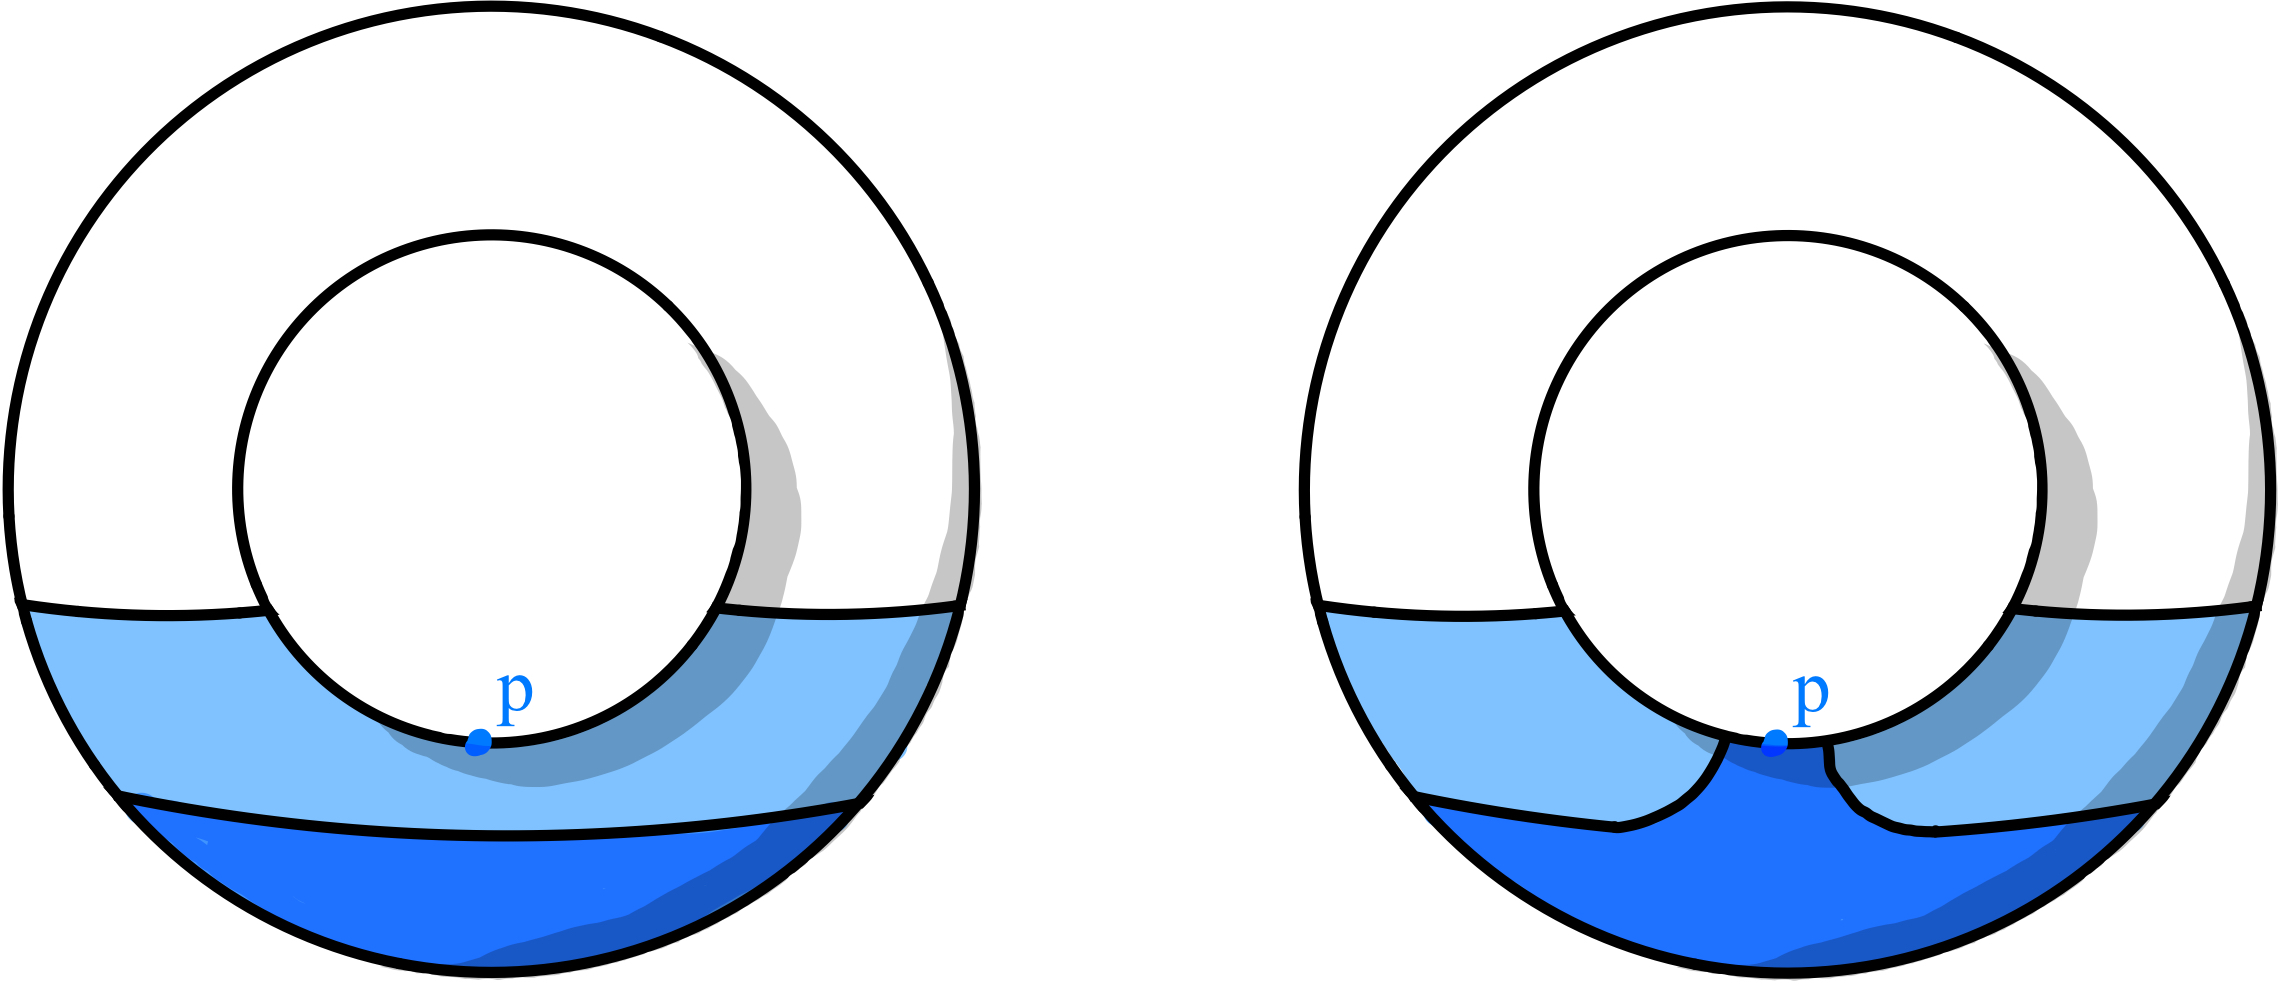
\includegraphics[width=0.8\linewidth]{../resources/Me-Diagram5-sublevelsets-of-f-and-F.jpeg}
    \label{fig:me-diagram5}
    \caption{Die Niveaumengen von $f$ (links) und $F$ (rechts)}
\end{figure}

Wir wollen also, dass $M^{c + \varepsilon} = F^{-1}(- \infty, c + \varepsilon]$ 
gilt und $F^{-1}(-\infty, c - \varepsilon]$ fast dasselbe ist wie 
$M^{c - \varepsilon}$, nur dass $F^{-1}(-\infty, c - \varepsilon]$ einen "Henkel"
enthält der den kritischen Punkt $p$ enthält.

\begin{bigproof}[Beweis zweites Deformationslemma]
    Sei $c := f(p)$. Mit dem Morse-Lemma können wir lokale Koordinaten 
    $\varphi = (u_1, ..., u_n)$ in einer Umgebung $U$ von $p$ wählen, sodass
    \[ f = c - u_1^2 - ... - u_k^2 + u_{k+1}^2 + ... + u_n^2 \]
    in dieser Umgebung, und sodass für den kritischen Punkt $p$ gilt:
    \[ u_1(p) = ... = u_n(p) = 0 \]

    Sei oBdA. $\varepsilon > 0$ klein genug, sodass 
    \begin{enumerate}
        \item $f^{-1}[c - \varepsilon, c + \varepsilon]$ kompakt ist und keine
            kritischen Punkte außer $p$ enthält
        \item $\{ x \in \R^n: \lVert x \rVert^2 \leq 2 \varepsilon \} \subseteq \varphi(U) $
    \end{enumerate}

    Wähle nun die $k$-Zelle 
    \[ 
        e^k := \{ p \in M: (u_1(p))^2 + ... + (u_k(p))^2 \leq \varepsilon 
        \text{ und } u_{k+1}(p) = ... = u_n(p) = 0 \} 
    \]

    Wir bekommen die folgende Situation:

    \begin{figure}[H]
        \centering
        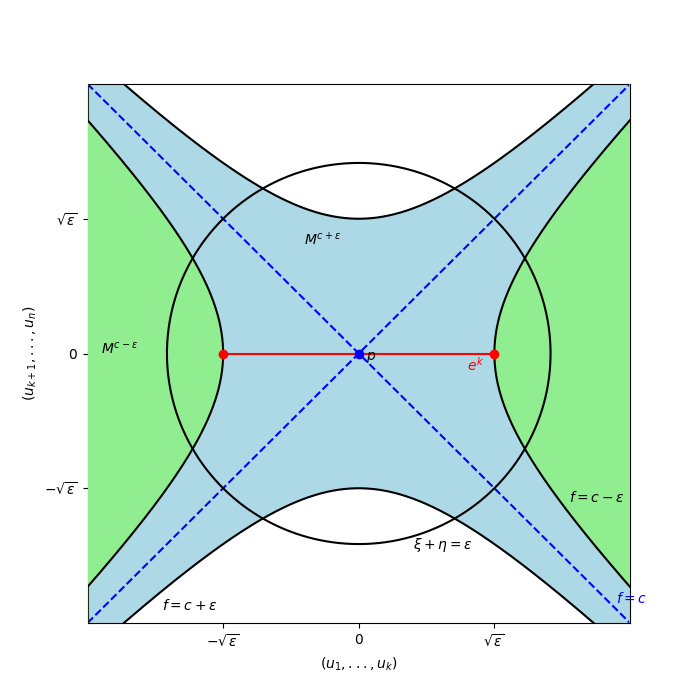
\includegraphics[width=0.8\linewidth]{../resources/Me-Diagram6-U-parameterized.png}
        \label{fig:me-diagram6}
        \caption{U parametrisiert}
    \end{figure}

    Nun definiere eine glatte Funktion $\mu: \R \to \R$ mit den Eigenschaften:

    \begin{enumerate}
        \item $ \mu(0) > \varepsilon $
        \item $ \mu(r) = 0 $ falls $ r \geq 2 \varepsilon $
        \item $ -1 < \mu'(r) \leq 0 $ für alle $ r \in \R $
    \end{enumerate}

    Sei nun $F$ außerhalb von $U$ gleich $f$, und sei
    \[ F = f - \mu(u_1^2 + ... + u_k^2 + 2u_{k+1}^2 + ... + 2u_n^2) \]

    $F$ ist wohldefiniert und glatt, da $F$ außerhalb des Kreises mit Radius 
    $\sqrt{2\varepsilon}$ mit $f$ übereinstimmt und der gesamte Kreis in $U$ 
    enthalten ist. Damit haben wir einen guten Kandidaten foür $F$ gefunden.

    Wir definieren nun

    \begin{align*}
        & \eta, \xi: U \to [0, \infty) \\
        & \xi = u_1^2 + ... + u_k^2 \\
        & \eta = u_{k + 1}^2 + ... + e_n^2
    \end{align*}

    Dann gilt innerhalb von $U$:
    \[ f = c - \xi + \eta \]
    und 
    \[ F = f - \mu(\xi + 2 \eta) = c - \xi + \eta - \mu(\xi + 2 \eta) \]

    Jetzt wollen wir überprüfen:
    \begin{enumerate}
        \item $F^{-1}(-\infty, c + \varepsilon] = M^{c + \varepsilon}$.
        \item $F^{-1}(-\infty, c - \varepsilon]$ ist ein Deformationsretrakt von 
            $M^{c + \varepsilon}$.
        \item $M^{c - \varepsilon} \cup e^k$ ist ein Deformationsretrakt von
            $F^{-1}(-\infty, c - \varepsilon]$.
    \end{enumerate}

    Dann folgt schon die Behauptung.

    \begin{claim} 
        $F^{-1}(-\infty, c + \varepsilon] = M^{c + \varepsilon}$
    \end{claim}

    \begin{smallproof}
        Sei $q \in M$. Falls gilt $\xi(q) + 2 \eta(q) > 2 \varepsilon$ gilt 
        $F(q) = f(q) - \mu(\xi(q) + 2\eta(q)) = f(q)$,
        also gelte oBdA.
        \[ \xi(q) + 2 \eta(q) \leq 2 \varepsilon \]
        Dann:
        \[ F(q) \leq f(q) = c - \xi(q) + \eta(q) \leq c + \frac{1}{2}\xi(q) + \eta(q) \leq c + \varepsilon \]
    \end{smallproof}

    \begin{claim} 
        $F^{-1}(-\infty, c - \varepsilon]$ ist ein
        Deformationsretrakt von $M^{c + \varepsilon}$.
    \end{claim}

    \begin{smallproof}
        Bemerke: Die kritischen Punkte von $F$ stimmen mit denen von $f$ überein, 
        denn:

        \[ \pderive[F]{\xi} = -1 - \mu'(\xi + 2\eta)  < 0 \]
        und
        \[ \pderive[F]{\eta} = 1 - 2 \mu'(\xi + 2\eta) \geq 1 \]
        Insbsondere sind diese beiden Ableitungen also niemals $0$. Da 
        \[ \opd F = \pderive[F]{\xi}\opd \xi + \pderive[F]{\eta} \opd \eta \]
        und $\opd \xi$ und $\opd \eta$ nur in $p$ gleichzeitig Null sind, haben $f$ 
        und $F$  dieselben kritischen Punkte.

        Betrachte die Region $F^{-1}[c - \varepsilon, c + \varepsilon]$. Wegen 
        Behauptung 1 und der Tatsache, dass $F \leq f$ gilt:
        \[ F^{-1}[c - \varepsilon, c + \varepsilon] \subseteq f^{-1}[c - \varepsilon, c + \varepsilon] \]
        Da $f^{-1}[c - \varepsilon, c + \varepsilon]$ kompakt ist und 
        $F^{-1}[c - \varepsilon, c + \varepsilon]$ abgeschlossen ist, ist 
        $F^{-1}[c - \varepsilon, c + \varepsilon]$ auch kompakt. Da $f$ und $F$
        dieselben kritischen Punkte haben kann diese Menge maximal den kritischen 
        Punkt $p$ enthalten, aber
        \[ F(p) = c - \xi(p) + \eta(p) + \mu(\xi(p) + 2\eta(p)) = c - \mu(0) < c - \varepsilon \]
        Also gibt es in $F^{-1}[c - \varepsilon, c + \varepsilon]$ keine kritischen
        Punkte. Mit dem ersten Deformationslemma gilt dann:
        $F^{-1}(- \infty, c - \varepsilon]$ ist Def. Retrakt von 
        $F^{-1}(-\infty, c + \varepsilon] = M^{c + \varepsilon}$.
    \end{smallproof}

    \begin{claim}
        $M^{c - \varepsilon} \cup e^{k}$ ist ein 
        Deformationsretrakt von $F^{-1}(-\infty, c - \varepsilon]$.
    \end{claim}

    \begin{smallproof}
        Diese Aussage ergibt nur Sinn, falls 
        $M^{c - \varepsilon} \cup e^{k} \subseteq F^(-\infty, c - \varepsilon]$.
        Wir wissen schon, dass $M^{c - \varepsilon} \subseteq F^{-1}(c - \varepsilon]$.

        Sei $q \in e^k$, dann gilt $\xi(p) = 0 \leq \xi(q) \leq 1$ und 
        $\eta(p) = 0 = \eta(q)$. Da 
        $\pderive[F]{\xi} < 0$ gilt dann
        \[ F(q) \leq F(p) < c - \varepsilon \]

        Also ergibt sich folgende Situation:

        \begin{figure}[H]
            \centering
            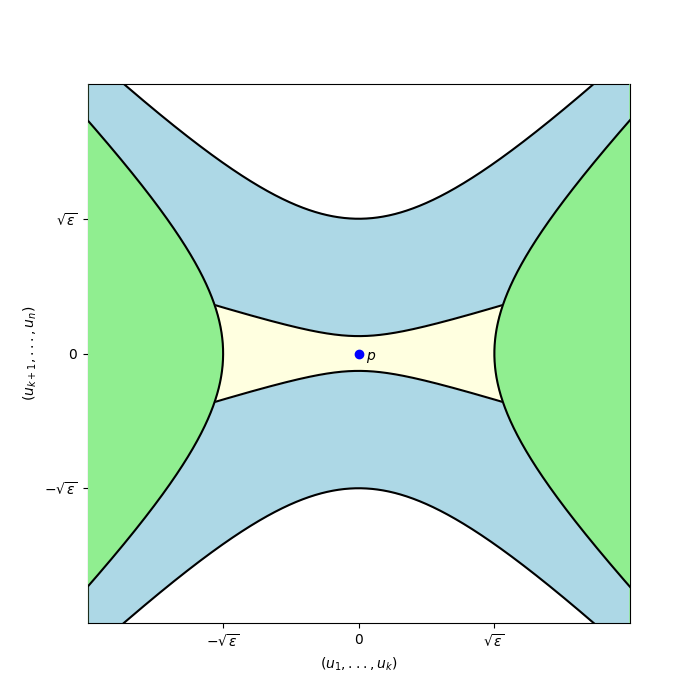
\includegraphics[width=0.8\linewidth]{../resources/Me-Diagram7-handle.png}
            \label{fig:me-diagram7}
            \caption{Henkel}
        \end{figure}

        Die hellgrün eingefärbte Fläche ist $M^{c - \varepsilon}$ die hellgelbe
        zusammen mit der hellgrünen Fläch ist $F^{-1}(-\infty, c - \varepsilon]$. 

        Dafür konstruieren wir eine Deformationsretraktion
        $r: F^{-1}(-\infty, c - \varepsilon] \times [0,1] \to F^{-1}(-\infty, c - \varepsilon]$
        für $q \in F^{-1}(-\infty, c - \varepsilon], t \in [0, 1]$, die 
        $F^{-1}(-\infty, c - \varepsilon] - M^{c - \varepsilon}$ auf $e^k$ 
        deformiert, wie folgt.

        \[
            r(q, t) = \begin{cases}
                \varphi^{-1} \circ (u_1, ..., u_k, tu_{k + 1}, ..., tu_n)(q)
                    & \text{ im Fall 1: } \xi(q) \leq \varepsilon \\
                \varphi^{-1} \circ (u_1, ..., u_k, s_tu_{k + 1}, ..., s_tu_n)(q)
                    & \text{ im Fall 2: } \varepsilon \leq \xi(q) \leq \eta(q) + \varepsilon \\
                q & \text{ im Fall 3: } \eta(q) + \varepsilon \leq \xi(q)
            \end{cases}
        \]

        Wobei 

        \[ s_t = t + (1 -t)((\xi - \varepsilon)/\eta)^{1/2} \]

        Die Fälle sind dann wie folgt:

        \begin{figure}[H]
            \centering
            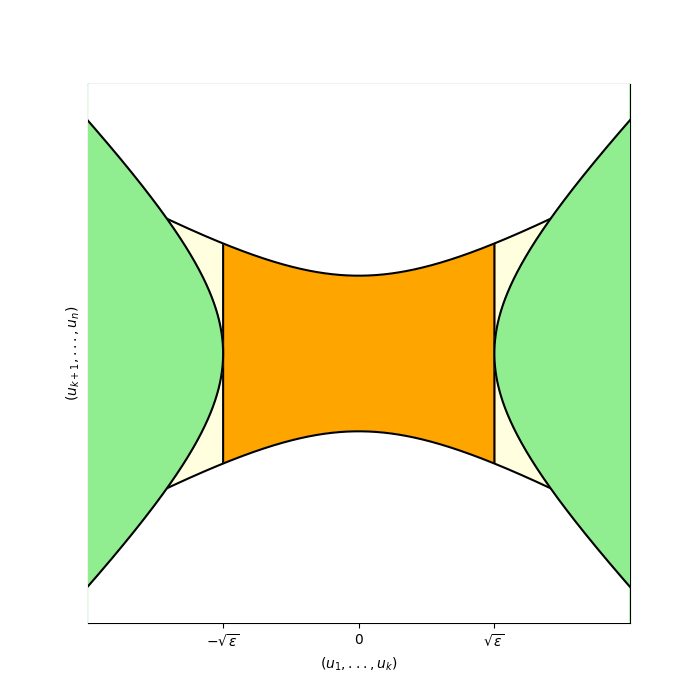
\includegraphics[width=0.8\linewidth]{../resources/Me-Diagram9-handle-cases.png}
            \label{me-diagram9}
            \caption{
                Fall 3 ist $M^{c - \varepsilon}$, also die grün eingefärbte Fläche, die
                orangene Fläche ist Fall 1 und die gelbe ist Fall 2.
            }
        \end{figure}

        Wir müssen überprüfen:
        \begin{enumerate}
            \item $r$ ist wohldefiniert und stetig
            \item $r(F^{-1}(-\infty, c - \varepsilon], 0) \subseteq M^{c - \varepsilon} \cup e^k$
            \item $r(\cdot, 1) = \id_{F^{-1}(-\infty, c - \varepsilon]}$ und 
                $\left. r(\cdot , 0) \right\vert_{M^{c - \varepsilon} \cup e^k} 
                = \id_{M^{c - \varepsilon} \cup e^k}$
        \end{enumerate}

        3. ist einfach nachzurechnen. In Fall 1 und Fall 3 ist 2. offensichtlich
        wahr. Für Fall 2 gilt:
        \begin{align*} 
            f(r(0, q)) & = 
                f\left( \varphi^{-1} \left(u_1(q), ..., u_k(q), 
                \left( \frac{\xi(q) - \varepsilon}{\eta(q)} \right)^{1/2}u_{k + 1}(q), ...,
                \left( \frac{\xi(q) - \varepsilon}{\eta(q)} \right)^{1/2}u_n(q)
                \right)
                \right) \\
            & = c - \xi(q)
                + \left( \left( \frac{\xi(q) - \varepsilon}{\eta(q)} \right)^{1/2}u_{k + 1}(q) \right)^2 + ... 
                + \left( \left( \frac{\xi(q) - \varepsilon}{\eta(q)} \right)^{1/2}u_n(q) \right)^2 \\
            & = c - \left( \frac{\xi(q) - \varepsilon}{\eta(q)} \right) \eta(q) \\
            & = c - \varepsilon
        \end{align*}
        also ist $r(0, q) \in f^{-1}(c - \varepsilon)$. Um 1. zu prüfen müssen wir 
        Stetigkeit in den Grenzfällen überprüfen:
        \begin{align*}
            & \text{For } \xi(q) = \varepsilon \text{ : }
                & s_t(q)  =t + (1 - t)((\varepsilon - \varepsilon)/\eta(q))^{1/2} = t \\
            & \text{For } \eta(q) + \varepsilon = \xi(q) \text{ : }
                & s_t(q) = t + (1 - t)((\xi(q) - \varepsilon)/(\xi(q) - \varepsilon))^{1/2} = 1
        \end{align*}

        Das einzig andere Problem was wir bekommen könnten ist nun in Fall 2 falls
        $\eta \to 0$. In Fall 1 und Fall 3 bekommen wir für $q$ mit $\eta(q) = 0$:
        $r(q, t) = \varphi^{-1} \circ (u_1, ..., u_k, 0, ..., 0)(q)$, also wollen
        wir zeigen dass für $\eta \in $ Fall 2 mit $\eta \to 0$ gilt $s_tu_i \to 0$
        für $i \in \{k+1, ..., n\}$. In Fall 2 gilt
        $0 \leq \xi - \varepsilon \leq \eta$. Dann gilt:

        \begin{align*}
            \lim\limits_{\eta \to 0} | s_t u_i |
            & = \lim\limits_{\eta \to 0} (1 - t)((\xi - \varepsilon)/\eta)^{1/2} | u_i | \\
            & \leq \lim\limits_{\eta \to 0} (1 - t)(\eta/\eta)^{1/2}|u_i| \\
            & = \lim\limits_{\eta \to 0} (1 - t)|u_i| = 0 
        \end{align*}
        
        Also ist $r$ stetig.
    \end{smallproof}

    Mit Behauptung 3 und 4 bekommen wir
    \[ M^{c + \varepsilon} \simeq F^{-1}(c - \varepsilon] \]
    und 
    \[ F^{-1}(-\infty, c - \varepsilon] \simeq M^{c - \varepsilon} \cup e^k \]
    Also folgt die Behauptung:
    \[ M^{c + \varepsilon} \simeq M^{c - \varepsilon} \cup e^k \]

\end{bigproof}


\chapter{Der Morse-Komplex}
dfgdfgdfg
In diesem Kapitel wird der Morse Komplex definiert und gezeigt, dass der 
Morse-Komplex ein Kettenkomplex ist.

\section{Die stabile- und instabile Mannigfaltigkeit und die Smale-Bedingung}

\begin{definition}[Stabile- und instabile Mannigfaltigkeit]
    \label{def: stabile und instabile mannigfaltigkeit}
    Es sei $f \colon M \to \R$ eine Morse-Funktion, $p$ ein kritischer Punkt von $f$ und $X$ ein
    Pseudo-Gradientenfeld von $f$. Die stabile Mannigfaltigkeit von $f$ ist die Menge
    \[ \stab (p) = \left\{ q \in M : \lim_{t \to + \infty} \phi_t(q) = p \right\} \]
    und die instabile Mannigfltigkeit ist
    \[ \unst (p) = \left\{ q \in M : \lim_{t \to - \infty} \phi_t(q) = p \right\} . \]
\end{definition}

Bevor wir die stabile- und instabile Mannigfaltigkeit eines kritischen Punktes weiter untersuchen, 
fixieren wir ein Paar Notationen zu Morse Umgebungen.

\begin{definition}[Notationen zu Morse Umgebungen]
    \label{def: notation morse umgebung}
    Zuerst untersuchen wir eine quadratische Form, die die Form hat wie Funktionen in Morse
    Umgebungen, also
    \[ Q \colon \R^n \to \R ; Q(x_1, \dots, x_n) = - x_1 - \dots - x_k + x_{k + 1} + \dots + x_n \]
    für ein $1 \leq k \leq n$.
    Mit $x_- := (x_1, \dots x_k) \colon \R^n \to \R^k$ und $x_+ := (x_{k + 1} \dots x_n)$ gilt dann
    \[ Q = - \| x_- \|^2 + \| x_+ \|^2 . \]
    Der Gradient von $Q$ ist mit dem Standardskalarprodukt auf $\R^n$
    \[ \grad Q (x_-, x_+) = 2(x_-, x_+) . \]
    Seien nun $\eps, \eta > 0$. Dann setzen wir
    \[ U(\eps, \eta) := \left\{ x \in \R^n : - \eps < Q(x) < \eps 
    \text{ und } \| x_- \|^2 \| x_+ \|^2 \leq \eta(\eps + \eta) \right\} := U \]
    Wir definieren außerdem
    \begin{align*}
        \del_{\pm} U := & \left\{ x \in U: Q(x) = \pm \eps \text{ und } \|x_{\mp} \|^2 \leq \eta \right\} 
            \text{ und} \\
        \del_0 U := & \left\{ x \in \del U: \| x_- \|^2 \| x_+ \|^2 = \eta(\eps + \eta) \right\} .
    \end{align*}
    Dann gilt 
    \[ \del U = \del_+ \cup \del_- \cup \del_0 . \]
    Wir setzen nun $V_- = \langle e_1, \dots, e_k \rangle$ und 
    $V_+ = \langle e_1, \dots, e_n \rangle \subseteq \R^n$. $V_+$ ist der größte Vektorraum, 
    auf dem $Q$ positiv definit ist und $V_-$ der größte Vektorraum, auf dem $Q$ negativ definit ist. 
    Es gilt 
    \[ \del U \cap V_{\pm} \subseteq \del_{\pm} U . \]

    Ist nun $f \colon M \to \R$ eine Morse Funktion, $p$ ein kritischer Punkt von $f$ und $(U, \phi)$
    eine Morse Umgebung von $p$, dann hat $\phi \circ (f - f(p))$ auf $U$ genau die Form von $Q$, wenn
    $k$ der Index von $p$ ist. Dann gilt 
    \[ 
        \phi(\stab(p) \cap U) = V_- \cap \phi(U) \text{ und } 
        \phi(\unst(p) \cap U) = V_+ \cap \phi(U) .
    \]
\end{definition}

Wir sind nun bereit eine grundlegende aber wichtige Aussage zu beweisen.

\begin{prop}
    Ist $f \colon M \to \R$ eine Morse Funktion und $p$ ein kritischer Punkt von $f$, dann sind
    $\stab (p)$ und $\unst (p)$ Mannigfaltigkeiten mit 
    \[ \dim \unst (p) = n - \dim \stab (p) = \Index (p) \]
\end{prop}

\begin{proof}
    Es sei $(\psi, V)$ eine Morse Karte um $p$ in einer Form wie in ~\ref{def: notation morse umgebung},
    also sodass $\eps, \eta > 0$ exitstieren, sodass $\psi(V) = U(\eps, \eta) := U$. Es sei außerdem
    $\phi$ der Fluss eines Pseudo-Gradientenfeldes von $f$. Dann ist 
    \[ \Phi \colon \psi^{-1}(\del_+ U \cap V_+) \times \R \to M ; \psi(q, t) = \phi_t(q) \]
    eine Einbettung und es gilt 
    \[ \stab (p) = \Ima \Phi \cup \psi^{-1}(U \cap V_+) . \]
    Tatsächlich ist 
    \[ \stab (p) - \Ima \Phi = \{ p \} . \]
    Außerdem ist $\del_+ U \cap V_+ = \{ x \in \R^n: \| x_+ \|^2 = \eps \} \isom S^{n - k - 1}$, 
    denn für alle $x \in V_+$ gilt sowieso schon $x_- = 0$. Also ist $ \stab(p)$ diffeomorph zum Raum 
    $S^{n - k - 1} \times (-\infty, \infty]/\sim$, in dem alle Punkte in $\infty$ zusammengeklebt 
    werden. Dieser Quotient ist wiederum diffeomorph zur offenen Kreisscheibe mit Dimension $n - k$.
    Genauso zeigt man, dass $W^u (p)$ diffeomorph zur offenen Kreisscheibe mit Dimension $k$ ist.
\end{proof}

\begin{prop}
    \label{prop: trajektorien enden in kritischen punkten}
    Es sei $f \colon M \to \R$ eine Morse-Funktion und $X$ ein Pseudo-Gradientenfeld von $f$. 
    Sei außerdem $M$ kompakt. Ist dann $\phi$ der Fluss von $X$, dann existieren für jeden Punkt 
    $p \in M$ kritische Punkte $q$ und $r$ von $f$, sodass
    \[ \lim_{t \to + \infty} \phi_t(p) = q \;\;\; 
    \text{ und } \;\;\; \lim_{t \to -\infty} \phi_t(p) = r \]
\end{prop}

\begin{proof}
    Wir zeigen die erste Aussage. Seien für kritische Punkte $q$ $(U_q, \psi_q)$ die Karten, 
    auf denen der Pseudo Gradient mit dem negativen Gradienten auf $\R^n$ übereinstimmt. 
    Es ist $\lim_{t \to + \infty} \phi_t(p) = q$, genau dann wenn
    der Fluss $\phi_{\bullet}(p)$ den Punkt $p$ irgendwann in die Umgebung 
    $\del_+\psi_q(U_q) \cap \stab(q)$ transportiert. Angenommen $\phi_{\bullet}(p)$ transportiert
    $p$ nie zu einem kritischen Punkt. Jedes mal wenn $\phi_{\bullet}(p)$ also ins Innere einer
    Morse-Umgebung $U_q$ gerät, muss diese Umgebung auch wieder verlassen werden. Da 
    $f \circ \phi_{bullet}(p)$ monoton ist, kann nachdem $\phi_{bullet}(p)$ die Morse-Umgebung $U_q$
    verlassen hat, nie wieder zu dieser zurückgekehrt werden.
    Sei also 
    \[ U = \bigcup_{q \in \Crit(f)} U_q \]
    und $t_0$ der Zeitpunkt an dem $\phi_{\bullet} (p)$ die Umgebung $U$ das letzte mal verlässt.
    Da $M - U$ keine kritischen Punkte von $f$ enthält existiert ein $\eps_0 > 0$, sodass für alle 
    $x \in M - U$ gilt 
    \[ \opd f (x) ((X(x))) \leq - \eps_ . \]
    Wir rechnen also: Für jedes $t \geq t_0$ gilt
    \begin{align*}
        f(\varphi_t(p) - f(\varphi_{t_0}(p))) = & 
            \int_{t_0}^t \derive[f \circ \phi_{\bullet}(p)]{s} (s) \opd s \\
        = & \int_{t_0}^t \opd f (\phi_s(p)) (X(\phi_s(p))) \opd s \\
        \leq & - \eps_0 (t - t_0) . 
    \end{align*}
    Also für $t \to + \infty$ gilt $f(\phi_t(p)) \to - \infty$. Das kann aber nicht sein, denn da 
    $M$ kompakt ist muss auch $\Ima f$ kompakt sein. Also kann $\phi_{\bullet}(p)$ nicht alle 
    $U_q$ verlassen. aber dann ist 
    \[ \lim_{t \to + \infty} \phi_t(p) = q \]
    für einen kritischen Punkt $q$.
    Genauso zeigt man, dass $\lim_{t \to - \infty} \phi_t(p) = r$ für einen kritischen Punkt $r$.
\end{proof}

\begin{definition}[Smale-Bedingung]
    \label{def: smale-bedingung}
    Es sei $M$ eine Mannigfaltigkeit und $U$ und $V$ Untermannigfaltigkeiten von $M$. Wir sagen 
    $U$ und $V$ sind \textit{transversal} und schreiben $U \pitchfork V$, falls für alle Punkte 
    $p \in U \cap V$ gilt 
    \[ T_pU + T_pV = T_pM . \]
    Ein Vektorfeld $X \in \VFs (M)$ heißt \textit{transversal} zur Untermannigfaltigkeit $U$, falls 
    für alle $p$ in $U$ gilt 
    \[ \langle X(p) \rangle + T_pU = T_pM . \]

    Sei nun $f \colon M \to \R$ eine Morse Funktion und $X$ ein Pseudo-Gradientenfeld von $f$. Dann sagen
    wir, dass $X$ die \textit{Smale-Bedingung} erfüllt, falls für alle kritischen Punkte $p$ und $q$ von 
    $f$ gilt 
    \[ \stab (p) \pitchfork \unst (q) . \]
    Ein Paar $(f, X)$ aus einer Morse-Funktion $f$ und einem Pseudo-Gradientenfeld $X$, das die 
    Smale-Bedingung erfüllt, nennt man \textit{Morse-Smale Paar}.
\end{definition}

\begin{prop}
    Sind $U_1$ und $U_2$ Untermannigfaltigkeiten von einer $n$-\\
    dimensionalen Mannigfaltigkeit $M$ mit 
    Dimensionen $d_1$ und $d_2$, sodass 
    \[ U_1 \pitchfork U_2 , \]
    dann ist $U_1 \cap U_2$ eine Untermannigfaltigkeit von $M$ mit Dimension $d_1 + d_2 - n$.
\end{prop}

\begin{proof}
    Fixiere einen Punkt $p \in U_1 \cap U_2$. Da $U_1$ und $U_2$ Untermannigfaltigkeiten sind existieren 
    Karten $(\phi_1, V_1)$ und $(\phi_2, V_2)$ von $M$, sodass 
    \[ \phi_1 = (\phi_1', \phi_1'') \colon V_1 \to 
        \Omega_1 \times \Omega_1' \subseteq \R^{d_1} \times \R^{n - d_1} \]
    mit $\phi_1(V_1 \cap U_1) = \Omega_1 \times \{ 0 \}$ und 
    \[ \phi_2 = (\phi_2', \phi_2'')\colon V_2 \to 
        \Omega_2 \times \Omega_2' \subseteq \R^{d_2} \times \R^{n - d_2} \]
    mit $\phi_2(V_2 \cap U_2) = \Omega_2 \times \{ 0 \}$. Definiere 
    \[ \phi'' = (\phi_1'', \phi_2'') \colon 
        M \supseteq V_1 \cap V_2 \to \R^{n - d_1} \times \R^{n - d_2}. \]
    Dann ist 
    $(\phi'')^{-1}(0) = (U_1 \cap V_1) \cap (U_2 \cap V_2) = (U_1 \cap U_2) \cap (V_1 \cap V_2) := V$.
    Wir wollen nun den Satz über reguläre Werte anwenden, aber dafür müssen wir zeigen, dass 
    $\opd_p \phi''$ surjektiv ist. Bemerke, dass 
    $\opd_p \phi'' = \opd_p (\phi''_1, \phi''_2) = (\opd_p \phi''_1, \opd_p \phi''_2)$.
    Es sei $v \in T_p\R^{n - d_1}$ und $w \in T_p\R^{n - d_2}$. Da $\opd_p \phi''_1$ und 
    $\opd_p \phi''_2$ surjektiv sind, und da $U_1$ und $U_2$ transversal sind, 
    existieren $v_1' + v_2', w_1' + w_2' \in T_pU_1 + T_pU_2$, sodass 
    $\opd_p \phi''_1 (v_1 + v_2) = \opd_p \phi''_1 (v_2) = v$ und 
    $\opd_p \phi''_2 (w_1 + w_2) = \opd_p \phi''_2 (w_1) = w$.
    Die ersten Gleichheiten gelten, da $T_pU_1$ der Kern von $\opd \phi''_1$ und 
    $T_pU_2$ der Kern von $\opd \phi''_2$ sind. Dann gilt
    \[ \opd_p \phi'' (w_1' + v_2')  = ( \opd_p \phi''_1 (v_2'), \opd_p \phi''_2 (w_1')) = (v, w) . \]
    Wir können also den Satz über reguläre Werte anwenden, dann ist $V$ eine Untermannigfaltigkeit
    mit Dimension $n - ((n - d_1) + (n - d_2)) = d_1 + d_2 - n$. Dann ist auch $U_1 \cap U_2$
    eine Untermannigfaltigkeit von Dimension $d_1 + d_2 - n$.
\end{proof}

Dann folgt direkt:

\begin{prop}
    Es sei $f \colon M \to \R$ eine Morse Funktion und $p$ und $q$ kritische Punkte von mit Index $k_1$
    und $k_2$ respektive. Falls $X$ die Smale-Bedingung erfüllt ist
    \[ \mathcal{M} (p, q) := \unst (p) \cap \stab (q) = 
        \left\{ r \in M : \lim_{t \to - \infty} \phi_t(p) \text{ und } 
        \lim_{t \to + \infty} \phi_t(q) \right\} \]
    ist eine Mannigfaltigkeit mit Dimension $k_1 - k_2$.
\end{prop}

Der Raum $\mathcal{M} (p, q)$ beinhaltet alle Punkte, die Auf Trajektorien zwischen den kritischen
Punkten $p$ und $q$ liegen. 

\todo{Zeichnung}

\begin{prop}
    Ist $M$ kompakt, $f \colon M \to \R$ eime Morse Funktion, $p \neq q$ kritische Punkte mit Index
    $k_1, k_2$, dann wirkt $\R$ via $(p, t) \mapsto \phi_t(p)$ frei und eigentlich auf 
    $\mathcal{M} (p, q)$, also ist
    \[ \Lt (p, q) = \mathcal{M}(p, q)/\R \]
    eine $(k_1 - k_2 - 1)$-dimensionale Mannigfaltigkeit.
\end{prop}

\begin{proof}
    Die Abbildung 
    $\Phi \colon \mathcal{M} (p , q) \times \R \to \mathcal{M} (p, q) \times \mathcal{M} (p,q) ; 
    (p, t) \mapsto (p, \phi_t(p))$ ist glatt, denn da $M$ kompakt ist, ist $\phi$ eine 
    1-Parameter-Gruppe aus Diffeomorphismen (~\ref{prop: kompaktes VF generiert 1-param. grp.}). 
    Sei nun $I \subset \R$ ein kompaktes Intervall. 

    Die Gruppenwirkung ist frei, denn in $\mathcal{W} (p, q)$
    sind keine kritischen Punkte, da $p \neq q$. Es sei $x$ in $\mathcal{M} (p, q)$. 
    Ist nun $t \neq 0$, dann gilt da $f \circ \phi_{\bullet}$ streng monoton ist 
    $f(\phi_t(x)) \neq f(\phi_0(x))$, also $\phi_t(x) \neq x$.
\end{proof}

Der Raum $\Lt (p, q)$ enthält für jede Trajektorie, die zwischen den kritischen Punkten $p$ und $q$ 
verläuft einen Repräsentanten. Später wird $\Lt (p, q)$ benutzt, um den Morse-Lomplex zu definieren.
Die Smale Bedingung ist also für unsere Zwecke wichtig. 

Wir gewinnen auch eine wichtige Erkenntnis: 

\begin{corollary}
    Der Index von kritischen Punkten erhöht sich entlang von Trajektorien. Denn falls 
    $\Index (p) < \Index (q)$, dann ist die Dimension von $\mathcal{M} (p, q)$
    kleiner $0$, also ist dann $\mathcal{M} (p, q) = \varnothing$.
\end{corollary}

Um also den Morse Komplex für jede (kompakte) Mnnigfaltigkeit definieren zu können, müssen wir noch die 
Existenz von Morse-Smale Paaran zeigen. Sogar noch stärker ist die folgende Aussage:

\begin{theorem}[Satz von Smale-Kupta]
    Es sei $M$ eine Mannigfaltigkeit mit Rand  \\
    und $f$ eine Morse-Funktion, sodass $f|_{\Crit{f}}$ bijektiv ist. Es sei $\Omega$ die Vereinigung 
    von Morse-Umgebungen von allen kritischen Punkten. Sei $X$ ein Pseudo-Gradientenfeld von $f$. 
    Dann existiert ein Pseudo-Gradientenfeld $X'$ von $f$, das die Smale Bedingung erfüllt, das 
    innerhalb von $\Omega$ gleich $X$ ist und für das gilt:

    Für jedes $\eps > 0$, jeden Atlas $(\phi_i, U_i)_{i \in I}$ von $M$ und alle $i \in I$ existiert 
    für jede Kompakte Teilmenge $K_i \subseteq U_i$ ein Vektorfeld $X'$, sodass 
    \[ \| \opd \phi_i^{-1} (\cdot) (X') - \opd \phi_i^{-1} (\cdot) (X) \| < \eps . \]
\end{theorem}

\begin{proof}
    \todo{?} Der Beweis dieses Satzes ist zum Beispiel in \cite{audin} zu finden.
\end{proof}

\section{Der Morse-Komplex und der Raum der gebrochenen Trajektorien}

Wir sind nun bereit, den Morse-Komplex mit Koeffizienten in $\F_2$ (wenigstens) hinzuschreiben.
Wir fixieren für den gesamten Abschnitt eine glatte kompakte Mannigfaltigkeit $M$ und ein
Morse-Smale Paar $(f, X)$. Dann definiere
$C_k (M, (f, X))$ als das $\F_2$ Modul, das von den kritischen Punkten von $f$ mit Index $k$ 
erzeugt wird. Außerdem sei $n_X(p, q) = \# \Lt (p, q) \mod 2$. Dann definiere für einen kritischen Wert
$p$:
\[ \del_X (p) := \sum_{\substack{ q \in \Crit(f) \\ \Index (p) + 1 = \Index (q) }} \del_X(p, q)p . \]

Das Ziel dieses Abschnittes ist es zu zeigen, dass der Komplex $C_{\ast}(M, (f, X))$ ein Kettenkomplex
ist, also dass $\del_X \circ \del_X = 0$. 

Sind dafür $p$ und $q$ zwei kritische Punkte von $f$ mit $\Index (p) = \Index (q) + 2$, dann genügt es 
zu zeigen, dass $\# \Lt (p, q)$ gerade ist. Dafür benötigen wir folgende Konstruktion:

\begin{definition}[Der Raum der gebrochenen Trajektorien]
    \label{def: raum der gebrochenen trajektorien}
    Es seien $p$ und $q$ kritische Punkte von $f$. Der \textit{Raum der gebrochenen Trajektorien} ist
    \[ \Lb (p, q) = 
        \bigcup_{k \in \N} \left( \bigcup_{\substack{c_1, \dots, c_{k - 1} \\ \in \Crit(f)}} 
            \Lt (p, c_1) \times \Lt (c_1, c_2) \times \dots 
                \times \Lt (c_{k - 2}, c_{k - 1}) \times \Lt (c_{k - 1}, q) \right) . \]
\end{definition}

Obwohl die Formulierung recht sperrig wirkt ist sie doch intuitiv: 
$\ell \in \Lt (p, q)$ ist eine \glqq Verbindung\grqq{} zwischen den kritischen Punkten $p$ und $q$ 
entlang des Pseudo-Gradientenfeldes $X$. Ein Element 
$(\ell_1, ..., \ell_k) \in \Lt (p, c_1) \times \dots \times \Lt (c_{k - 1}, q) \subseteq \Lb (p, q)$
ist eine \glqq Verbindung\grqq{} zwischen $p$ und $q$ entlang des Pseudo-Gradientenfeldes $X$, die noch 
bei den kritischen Punkten $c_1, \dots, c_{k - 1}$ \glqq Halt\grqq{} macht. 

Offensichtlich gilt:
\begin{itemize}
    \item Ist $\Index (p) + 1 = \Index (q)$, so ist $\Lb (p, q) = \Lt (p, q)$.
    \item Ist $\Index (p) + 2 = \Index (q)$, so ist 
        $\Lb (p, q) = \Lt (p, q) \cup \bigcup_{c \in \Crit (f)} \Lt(p, c) \times \Lt(c, q)$
\end{itemize}

Wir werden sehen, dass man wie mit der Notation angedeutet $\Lb (p, q)$ mit einer Topologie ausstatten 
kann, sodass es die Kompaktifizierung von $\Lt (p, q)$ ist. (In der Tat ist ja 
$\Lt (p, q) \subseteq \Lb (p, q)$).

\begin{definition}[Topologie von $\Lb (p, q)$]
    Ese seien $p$ und $q$ kritische Punkte von $f$. Wir erinnern uns an unsere Vorstellung von Morse-
    Umgebungen $U = U(\eps, \eta)$ wie in~\ref{def: notation morse umgebung}:
    \begin{itemize}
        \item $\del_+ U$ sind alle Punkte auf dem Rand von $U$, auf denen Trajektorien von $X$ in 
            die Umgebung $U$ eintreten.
        \item $\del_- U$ sind alle Punkte auf dem Rand von $U$, auf denen Trajektorien von $X$ die
            Umgebung $U$ verlassen.
        \item Die Trajektorien von $X$ verlaufen tangential zu $\del_0 U$.
    \end{itemize}
    Es sei nun 
    \[ \ell = (\lambda_1, \dots, \lambda_k) 
        \in \Lt (p, c_1) \times \dots \times \Lt(c_{k - 1}, q) \subseteq \Lb (p, q) . \]
    Seien $U_i = U_i (\eps_i, \eta_i)$ Morse Umgebungen von $c_i$ und $U_0$ und $U_k$ Morse 
    Umgebungen von $p$ und $q$. $\lambda_i \cap \del_+ U_i$ ist der Punkt, an dem $\lambda_i$
    in $U_i$ eintritt, und $\lambda_{i + 1} \cap \del_- U_i$ ist der Punkt, an dem $\lambda_{i + 1}$
    die Umgebung $U_i$ verlässt. Es sei $U_i^-$ eine Umgebung von $\lambda_i \cap \del_+ U_i$ in 
    $\del_+ U$ und $U_i^-$ eine Umgebung von $\lambda_{i + 1} \cap \del_- U_i$ in $\del_- U_i$. 
    Seien dann $U^- = \bigcup U_i^-$ und $U^+ = \bigcup U_i^+$. Dann definiere die Menge 
    $\mathcal{U} (\ell, U^-, U^+)$ wie folgt:

    Wir sagen 
    $\ell' = (\mu_1, ..., \mu_{k'}) \in \Lt (p, c_{i_1}) \times \dots \times \Lt (c_{i_{k'-1}}, q)$
    ist in $\mathcal{U}(\ell, U^-, U^+)$ enthalten, falls $\mu_j \cap U_j^+ \neq \varnothing$
    und $\mu_j \cap U_{j + 1}^- \neq \varnothing$. 
    Dann ist $\mathcal{W} \subseteq \Lb (p, q)$ offen genau dann, wenn es für jedes 
    $\ell \in \mathcal{W}$ Umgebungen $U^+$ und $U^-$ wie oben gibt, sodass 
    $\mathcal{U}(\ell, U^+, U^-) \subseteq \mathcal{W}$.
\end{definition}

\begin{remark}
    Die Topologie von $\Lt(p, q)$ als Quotient stimmt mit der von $\Lb(p, q)$ überein.
    \todo{}
\end{remark}

\begin{prop}
    \label{prop: Lb ist kompakt}
    Es seien $p$ und $q$ kritische Punkte von $f$. Dann ist $\Lb (p, q)$ kompakt.
\end{prop}

Um diese Proposition zu beweisen benötigen wir noch ein Lemma:

\begin{lemma}
    \label{lemma: konvergenz einer folge}
    Es sei $x \in M$ \emph{kein} kritischer Punkt von $f$. Sei außerdem $(x_n)_n$ eine Folge in
    $M$ die gegen $x$ kovnvergiert und seien $y_n$ und $y$ Punkte, die auf den selben Trajektorien
    wie $x_n$ und $x$ liegen. Es gelte außerdem $f(y_n) = f(y)$ für alle $n \in \N$. Dann gilt
    \[ \lim_{n \to + \infty} y_n = y . \]
\end{lemma}

\begin{proof}
    Es sei $U$ eine Umgebung von $\Crit (f)$. Dann ist $\opd f (\cdot) (X)$ nie Null, und ähnlich wie 
    Im Beweis vom ersten Deformationslemma~\ref{satz: erstes deformationslemma} betrachten wir das
    Vektorfeld 
    \[ Y = - \frac{1}{\opd f (\cdot) (X)} \cdot X \]
    Auf $M - U$. Sei $\phi$ die von $Y$ erzeugte 1-Parameter Gruppe aus Diffeomorphismen. 
    Da $Y$ in die selbe Richtung zeigt wie $X$, stimmen die Trajektorien von $Y$ mit denen von $X$ 
    überein und es gilt 
    \[ f(\phi_t(z)) = f(z) - t . \]
    Dann gilt
    \[ \lim_{n \to \infty} y_n 
    = \lim_{n \to \infty} \phi_{- f(y_n) + f(x_n)}(x_n) 
    = \lim_{n \to \infty} \phi_{- f(y) + f(x_n)}(x_n) 
    = \phi_{- f(y) + f(x)}(x) = y \]
\end{proof}

\begin{proof}[Beweis von Proposition~\ref{prop: Lb ist kompakt}]
    Es sei $(\ell_n)_n$ eine Folge in $\Lb (p, q)$. Um zu zeigen, dass $Lb (p, q)$ kompakt ist
    müssen wir zeigen, dass $(l_n)_n$ eine konvergente Teilfolge besitzt.

    Wir nehmen zuerst an, dass für alle $n \in \N$ die Trajektorie $\ell_n$ in $\Lt (p, q)$.
    Seien $U$ und $V$ Morse Umgebungen von $p$ und $q$ in der Form wie bei der eingeführten
    Notation für Morse Umgebungen~\ref{def: notation morse umgebung}.
    Es außerdem sei $\ell_n^- \in M$ der Punkt, an dem $\ell_n$ die Morse Umgebung $U$ verlässt 
    und $\ell_n^- \in M$ der Punkt, an dem $\ell_n$ in die Morse Umgebung $V$ eintritt.
    $\ell_n^-$ und $\ell_n^+$ sind im Schnitt von $\del U$ bzw. $\del V$ und der stabilen bzw. 
    instabilen Mannigfaltigkeit. Diese Schnitte sind Kugeloberflächen, also kompakt. Die Folgen 
    $(l_n^-)_n$ und $(\ell_n^+)_n$ haben also konvergente Teilfolgen, wir können demnach ohne 
    Beschränkung der Allgemeinheit annehmen, dass sie konvergent sind. Setze
    \[ \lim_{n \to \infty} \ell_n^- = p^- \text{ und } \lim_{n \to \infty} \ell_n^+ = q^+ . \]
    Sei $\phi$ die von $X$ erzeugte 1-Parameter Gruppe aus Diffeomorphismen, dann ist 
    $\gamma = \phi_{\bullet}(p^-)$ die Trajektorie von $p^-$. Sei 
    $c = \lim_{n \to \infty} \phi_t(p^-)$. $c$ ist nach 
    Proposition~\ref{prop: trajektorien enden in kritischen punkten} ein kritischer Punkt,
    also ist $\gamma \in \Lt (p, c)$. Es sei nun $W$ eine Morse-Umgebung von $c$, die auch
    die Form hat wie in~\ref{def: notation morse umgebung}. Da $\phi$ glatt ist, muss für $n$ 
    groß genug auch $\ell_n$ die Morse Umgebung $W$ von $c$ kreuzen. Sei $d_n^+ \in M$ der Punkt, an
    dem $\ell_n$ in $W$ eintritt. Dann gilt $d_n^+, d^+ \in \del_+ W$, also gilt $f(d_n^+) = f(d^+)$
    für alle $n$. Da $d_n^+$ auf der selben trajektorie wie $p_n^-$ liegt, und $d^+$ auf der selben 
    Trajekorie wie $p^-$,folgt da $\lim p_n^- = p^-$ mit dem letzten 
    Lemma~\ref{lemma: konvergenz einer folge}: 
    \[ \lim_{n \to \infty} d_n^+ = d^+ . \]
    Falls $c = q$, dann ist $\lim \ell_n = \gamma \in \Lt (p, q) \subseteq \Lb (p, q)$, also hat 
    dann die Folge $(\ell_n)_n$ eine konvergente Teilfolge. Es sei also $c \neq q$. Dann muss 
    $\ell_n$ die Morse Umgebung $W$ wieder durch einen Punkt $d_n^-$ verlassen. Wie oben können wir 
    ohne Beschränkung der Allgemeinheit annehmen, dass die Folge $(d_n^-)_n$ konvergent ist, da
    sie zumindest eine konvergente Teilfolge besitzt. Wir definieren dann $d^- = \lim d_n^-$. 
    $d^-$ liegt in der instabielen Mannigfaltigkeit von $c$, denn wäre dies nicht der Fall, dann 
    führt das zu einem Widerspruch:
    
    Angenommen $d^- \notin \unst (c)$. Dann wäre $d^-$ auf der Trajektorie von einem Punkt
    $d^+_{\ast} \in \del_+ W$, der nicht in $\stab (c)$ enthalten ist. Wieder wegen des vorherigen
    Lemmas~\ref{lemma: konvergenz einer folge} ist dann $\lim d_n^+ = d^+_{\ast}$, also gilt dann
    $d^+ = d^+_{\ast}$, aber es gilt $d^+ \in \stab{c}$.
    
    Wir können nun wieder mit dem selben Argument zeigen, dass dann die Trajektorie von $d^-$ im
    kritischen Punkt $q$ endet, also liegt dann $\lim \ell_n$ in $\Lt (p, c) \times \Lt (c, q)$.

    Jetzt fehlt uns noch der allgemeine Fall. Wir müssen also für eine Folge $(\ell_n)_n$ in 
    $\Lb (p, q)$ zeine konvergente Teilfolge finden. Wegen der Glattheit von $\phi$ können wir annehmen,
    dass für $n$ groß genug alle $\ell_n$ die Form 
    \[ \ell_n = (\ell^1_n, \dots, \ell^k_n) \in \Lt (p, c_1) \times \dots \times \Lt (c_{k - 1}, q) \]
    haben. Wir finden mit der vorheringen Überlegung komponentenweise eine Teilfolge, sodass wir 
    für den grenzwert maximal noch $k - 1$ kritische Punkte als \glqq Zwischenstopp\grqq{} einfügen
    müssen. 
\end{proof}

\begin{theorem}[Klassifizierung kompakter 1-Mannigfaltigkeiten]
    Es sei $M$ eine kompakte zusammenhängende Mannigfaltigkeit mit Rand. Dann ist
    \begin{itemize}
        \item $M$ diffeomorph zu $S^1$, falls $\del M = \varnothing$
        \item $M$ diffeomorph zu $[0, 1]$, falls $\del M \neq \varnothing$
    \end{itemize}
\end{theorem}

\begin{proof}
    Betrachte zuerst den ersten Fall, also dass $M$ keinen Rand hat. Es sei 
    $\{ (U_1, \phi_1), \dots, (U_n, \phi_n) \}$ ein Atlas von $M$. Ohne Beschränkung der 
    Allgemeinheit können wir annehmen, dass alle $U_i$ zusammenhängend sind. 
    Da $M$ zusammenhängend ist, können wir außerdem annehmen, dass 
    $\bigcup_{i = 1}^k U_i$ für alle $k$ zusammenhängend ist. Dann existiert ein $1 \leq k < n$, 
    sodass $\bigcup_{i = 1}^k U_i$ diffeomorph zu $\R$ ist, aber $\bigcup_{i = 1}^{k + 1} U_i$ 
    nicht. Setze $U := \bigcup_{i = 1}^k U_i$ und $V = U_{k + 1}$. Seien $\phi \colon U \to \R$
    und $\psi \colon V \to \R$ Diffeomorphismen. 
    \begin{claim*}
        Ist $M = U \cup V$ eine 1-dimensionale Mannigfaltigkeit, $U$ und $V$ diffeomorph zu 
        $\R$, dann ist $M$ diffeomorph zu $S^1$ oder $\R$.
    \end{claim*}

    \begin{smallproof}
        Ohne Beschränkung der Allgemeinheit ist $U \not\subseteq V$ und \\ 
        $V \not\subseteq U$. Dann gibt es zwei Möglichkeiten:
        \begin{itemize}
            \item $\phi(U \cap V)$ und $\psi(U \cap V)$ sind offene Halbintervalle
            \item $\phi(U \cap V)$ und $\psi(U \cap V)$ sind jeweils die disjunkte Vereinigung
                zweier offener Halbintervalle
        \end{itemize}
        Im ersten Fall ist $M$ homeomorph zu $\R$:

        Wir dürfen annehmen, dass $\phi(U \cap V) = (- \infty, a)$ und $\psi(U \cap V) = (b, \infty)$,
        ansonsten ersetze $\phi$ mit $\-phi$ bzw. $\psi$ mit $-\psi$. Die Verkettung
        \[ \begin{tikzcd}
            (- \infty, a) = \phi(U \cap V) \arrow[r, "\phi^{-1}"] & 
                U \cap V \arrow[r, "\psi"] & 
                \psi(U \cap V) = (b, \infty)
        \end{tikzcd} \] 
        
        Ist insbesondere injektiv, also auch monoton wachsend. 
        \todo{}
    \end{smallproof}
\end{proof}


\chapter{Morse-Homologie und zelluläre Homologie}

In diesem Kapitel wird aus einem Morse-Smale Paar auf einer Mannigfaltigkeit
eine zelluläre Struktur dieser Mannigfaltigkeit konstruiert. Dann werden wir 
sehen, dass der Kettenkomplex, der von dieser Struktur induziert wird schon mit
dem Morse-Komplex übereinstimmt. Somit stimmt die Morse-Homologie mit der 
zellulären Homologie überein, also auch mit der singulären Homologie.

\section{CW-Komplexe}

\section{CW-Struktur von Mannigfaltigkeiten}

\section{Morse-Homologie ist zelluläre Homologie}

\section{Anwendungen}


\appendix

\chapter*{Anhang}

\begin{definition}[Mannigfaltigkeit \cite{ludwig}]
    \label{def: mannigfaltigkeit}
    Es sei $M$ ein topologischer Raum. 
    
    Eine \textit{Karte} von $M$ ist ein Tupel
    $(U, \varphi)$, wobei $U \subseteq M$ offen und $\varphi \colon U \to U' \in \R^n$ 
    ein Homeomorphismus ist.

    $\mathcal{A} = \left\{ (U_{\alpha}, \varphi_{\alpha}) \right\}_{\alpha \in I}$ ist ein 
    \textit{$n$-dimensionaler Atlas} von $M$ falls
    \begin{enumerate}
        \item $(U_{\alpha}, \varphi_{\alpha})$ ist eine Karte für jedes $\alpha \in I$
        \item $M = \bigcup_{\alpha \in I U_{\alpha}}$
    \end{enumerate}
    Ein Atlas ist $C^k$ für $k \in \{ \N_0 \cup \{ \infty, \omega \} \}$, falls für
    alle $\alpha, \beta \in I$ der \textit{Koordinatenwechsel} 
    \[ 
        \varphi_{\alpha \beta} := 
        \varphi_{\alpha} \circ \varphi_{\beta}^{-1} \colon 
        \varphi_{\beta} (U_{\alpha} \cap U_{\beta}) \to \varphi_{\alpha} (U_{\alpha} \cap U_{\beta})
    \]
    $C^k$ ist.
    
    Eine Karte $(U, \varphi)$ heißt \textit{$C^k$ kompatibel} mit einem $C^k$ Atlas 
    $\mathcal{A} = \left\{ (U_{\alpha}, \varphi_{\alpha}) \right\}_{\alpha \in I}$,
    falls für alle $\alpha \in I$ die Koordinatenwechsel $\varphi \circ \varphi_{\alpha}^{-1}$
    und $\varphi_{\alpha} \circ \varphi^{-1}$ $C^k$ sind.

    Eine \textit{$n$-dimensionale $C^k$ Mannigfaltigkeit} ist ein topologischer Raum $M$ 
    zusammen mit einem maximalen $C^k$ Atlas $\mathcal{A}$, sodass $M$ ein Hausdorff-Raum und
    zweitabzählbar ist. Maximal bedeutet hier, dass es keine mit $\mathcal{A}$ $C^k$ 
    kompatiblen Karten gibt, die nicht in $\mathcal{A}$ enthalten sind.

    Eine Mannigfaltigkeit heißt \textit{glatt} falls $k = \infty$.

    Für einen Punkt $p \in M$ und eine Karte $(\varphi, U)$ mit $p \in U$ 
    heißen $\varphi = (x_1, ..., x_n)$ \textit{lokale Koordinaten} um $p$.
\end{definition}

\begin{remark}
    Wenn der Atlas einer Mannigfaltigkeit angegeben wird, dann nie als maximaler Atlas.
    Es reicht ein Atlas, alle anderen Karten sind dann schon impliziert.
\end{remark}

\begin{definition}[Differenzierbarkeit]
    Sind $M, N$ $C^k$ Mannigfaltigkeiten, 
    $\mathcal{A} = (\varphi_{\alpha}, U_{\alpha})_{\alpha \in I}$ ein Atlas von $M$, 
    $\mathcal{B} = (\varphi_{\beta}, U_{\beta})_{\beta \in J}$ ein Atlas von $N$,
    dann heißt eine Abbildung $C^k$ oder \textit{$k$-mal differenzierbar}, falls für alle 
    $\alpha \in I$ und $\beta \in J$ die Abbildung
    \[ \psi_{\beta} \circ f \circ \varphi_{\alpha}^{-1} \colon \R^n \to \R^m \]
    $C^k$ ist.
\end{definition}

\begin{definition}[Tangentialraum]
    Der Tangentialraum einer $C^k$ Mannigfaltigkeit $M$ an einem Punkt $p \in M$ ist
    \[ T_pM := \left\{ X_p \colon C^{k} \to \R : X_p 
        \text{ ist eine Derivation von $M$ an dem Punkt $p$} \right\} \]
    Wobei $X_p: C^{k} \to \R$ ein \textit{Derivation} ist, falls folgende Bedingungen erfüllt
    sind:
    \begin{itemize}
        \item $X_p$ ist linear
        \item Für $X_p$ gilt die Leibnitz-Regel, also
            \[ X_p (f \cdot g) = X_p (f) \cdot g + f \cdot X_p (g) \]
    \end{itemize}
    Dann ist $T_pM$ ein Untervektorraum von $C^k(C^k(M))$.

    Für eine $C^k$ Abbildung $f \colon M \to N$  und einen Punkt $p \in M$ ist dann 
    \begin{align*}
        \opd f (p) \colon T_pM & \to T_{f(p)}N \\
        X_p & \mapsto f_* X_p
    \end{align*}
    wobei $f_*X_p$ definiert ist durch
    \[ f_*X_p (g) = X_p (g \circ f) \]
\end{definition}

\begin{remark}
    \begin{align*}
        T \colon \mathbf{Man}_{*} & \to \mathbf{Vect}_{\R} \\
        (M, p) & \mapsto T_pM \\
        f & \mapsto \opd f (p)
    \end{align*}
    Ist ein Funktor.
\end{remark}

\begin{remark}
    Es sei $M$ eine $C^k$ Mannigfaltigkeit, $k \geq 1$, $p \in M$ und $\varphi = (x_1, ..., x_n)$
    lokale Koordinaten um $p$. Definiere
    \begin{align*} 
        \pderive{x_1}(p): C^k(M) & \to \R \\
        \pderive[f]{x_i} (p) & = \pderive[\varphi \circ f]{x_i} (\varphi(p))
    \end{align*}
    Dann ist $\left( \pderive{x_i} \right)_{1 \leq i \leq n}$ eine Basis von $T_pM$.

    Für eine glatte Abbildung $f \colon M \to N$, einem Punkt $p \in M$ und lokale Koordinaten 
    $(x_1, ..., x_n)$ um $p$ und $(y_1, ..., y_m)$ um $f(p)$ bekommen wir in einer Umgebung 
    von $p$ wohldefinierte Abbildungen $f_i = y_i \circ f$. Dann ist das differential 
    $\opd f (p)$ von $f$ gegeben durch die Matrix
    \[ D_p(f) = \left( \pderive[f_i]{x_j} \right)_{i,j} . \]
\end{remark}



% \printbibliography

\eject
\end{document}